\documentclass{../template/tp}
\usepackage[utf8x]{inputenc}

\usepackage[frenchb]{babel}
\usepackage[T1]{fontenc}

\usepackage{graphicx}
\usepackage{amssymb}
\usepackage{amsmath}
\usepackage{wasysym} %smiley
\usepackage{hyperref}% hyperliens
\usepackage{tikz}
\usetikzlibrary{babel,positioning,calc}
\usepackage[]{circuitikz}
\usepackage{textcomp}
% \usepackage{minted}
\usepackage[long]{datetime}
\usepackage{gensymb} % \ohm, celsius
\usepackage{framed}
\usepackage{pdfpages}
\usepackage{todonotes}
\usepackage{enumitem}
\usepackage{ marvosym }
\usepackage{fancyhdr}
\usepackage{mathastext} % math as standfard text : units are respecting typography conventions.

% \langexam{frenchb}

\newboolean{koriG}
\ifx\koriG\undefined
\correction{false}
\else
\correction{true}
\fi

% \correction{false}
% \correction{true}

%% fancy header & foot
\pagestyle{fancy}
\lhead{[ELEC-H-301] Électronique appliquée\\ TP \no 4 : Diodes\ifthenelse{\boolean{corrige}}{~-- Corrigé}{}}
\rhead{v1.1.1\\ page \thepage}
\cfoot{}
%%

\pdfinfo{
/Author (Quentin Delhaye, ULB -- BEAMS)
/Title (TP 4 ELEC-H-301, diodes)
/ModDate (D:\pdfdate)

}
\hypersetup{
pdftitle={TP 4 [ELEC-H-301] Électronique appliquée : diodes},
pdfauthor={Ken Hasselmann, ©2016 ULB - BEAMS  },
pdfsubject={diodes}
}

\newcommand{\itgv}[1]{\ifthenelse{\boolean{corrige}}{\color{blue}#1}{}} %si corrigé vrai...
\newcommand{\ifgv}[1]{\ifthenelse{\boolean{corrige}}{}{#1}} %si corrigé faux...

\setlength{\parskip}{0.4cm plus4mm minus1mm} %espacement entre §
\setlength{\parindent}{0pt}

\author{The Fantastic Four}

\begin{document}

\tptitle{}{Séance 4~: Diodes}

\section*{Objectifs}
À la fin de cette séance d'exercices, vous serez en mesure de :
\begin{itemize}
\item comprendre les différentes modélisations des diodes (idéale, avec tension de seuil\dots)
\item résoudre des circuits à diodes utilisant différentes modélisations
\item calculer les différents éléments d'un régulateur à diode Zener
\end{itemize}

\section*{Exercices}
\Question{
Sur le schéma suivant :
\begin{itemize}
\item indiquer l'anode et la cathode de la diode
\item flécher et nommer les grandeurs électriques.
\end{itemize}
 Préciser les différents modèles électriques possibles pour la diode.
\\%
 Quelles sont les précautions à prendre lors de l'utilisation d'une diode ?
	\ifthenelse{\boolean{corrige}}{}{
		\begin{center}
		\begin{circuitikz}\draw
			(0,0) node[anchor=east] {} to [short] (1.5,0)
			(0,0) to [Do] (2.5,0) node [anchor=west]{}
		;\end{circuitikz}
		\end{center}
		}
}{
	\begin{center}
		\begin{circuitikz}\draw
			(0,0) node[anchor=east] {A} to [short,i>^=$I$] (1.5,0)
			(0,0) to [Do, v<=$V$] (2.5,0) node [anchor=west]{K}
		;\end{circuitikz}
	\end{center}

Modèles possibles pour la diode :
\begin{itemize}
	\item idéale : le \textbf{courant} circulant à travers la diode est \textbf{nul} si la diode est polarisée \textbf{en inverse}, la \textbf{tension} aux bornes de la diode est \textbf{nulle} si elle est polarisée \textbf{en direct} (par rapport au schéma ci-dessus, polarisation directe $\equiv V>0$).
	\item idéale avec tension de seuil :  le courant est nul si la diode est polarisée en inverse. Le courant est nul tant que la tension de seuil n'a pas été atteinte ($V_{TH}=0.7V$ habituellement). Si la diode est polarisée en direct \textbf{et} que la tension à ses bornes atteint $V_{TH}$, \textbf{alors} la diode est passante et un courant peut circuler à travers la diode. Quel que soit le courant($>0$), la tension aux bornes de la diode restera $V_{TH}$.
	\item idéale avec tension de seuil et résistance série : comme précédemment mais avec une résistance en série. Cette résistance modélise la résistance interne de la diode.
	\item exponentiel : ce modèle découle directement des caractéristiques électriques d'une jonction PN.
	\end{itemize}
	Le phénomène d'avalanche peut se modéliser de la même façon.

Précautions à prendre lors de l'utilisation d'une diode :
\begin{itemize}
\item quel que soit le mode de fonctionnement : ne jamais dépasser la puissance maximum que peut dissiper la diode
\item en direct : ne jamais dépasser le courant limite admissible par la diode. En particulier, ne jamais connecter une diode directement sur une source de tension
\item en inverse : ne jamais dépasser la tension d'avalanche, dans le cas d'une utilisation qui exclut tout fonctionnement en avalanche
\item en inverse : veiller à ne jamais dépasser le courant maximum admissible en inverse dans la zone d'avalanche (ce courant dépend de la puissance maximum admissible et de la tension d'avalanche de la diode).
\end{itemize}
}

\Question{%question
%storey 17.17
\begin{center}
    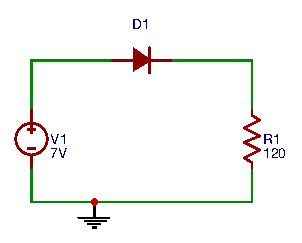
\includegraphics[scale=1.4]{1717}
\end{center}
Déterminer le courant dans ce circuit dans les deux cas suivants :
\begin{itemize}
    \item La diode est remplacée par une diode idéale.
    \item La diode est remplacée par une diode idéale en série avec une source de tension de 0.7~V.
\end{itemize}
Que se passe-t-il si on change le sens de la diode ?
}
{%answer
\begin{itemize}
    \item 1\ier~cas : $I = \frac{V_1}{R1} = \frac{7}{120} = 58.3mA$
    \item 2\ieme~cas : $I = \frac{V_1-V_{th}}{R1} = 52.5mA$ avec $V_{th}$ = 0.7V
\end{itemize}
Si on change le sens de la diode, celle-ci sera bloquante, par conséquent : $I=0$

}

% sedra 3.2 et 3.3
\Question{
\label{conti}
En considérant la diode comme idéale, calculer le courant circulant dans la résistance et la tension $V_o$ dans les circuits suivants.
\begin{center}
    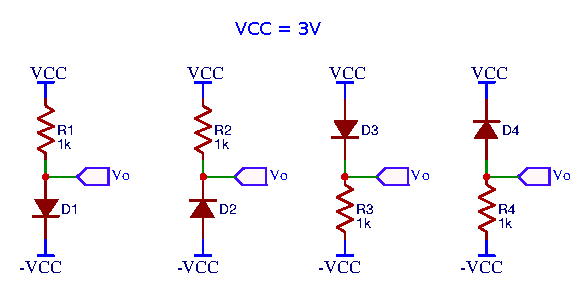
\includegraphics[scale=1.4]{ex2}
\end{center}
\begin{center}
    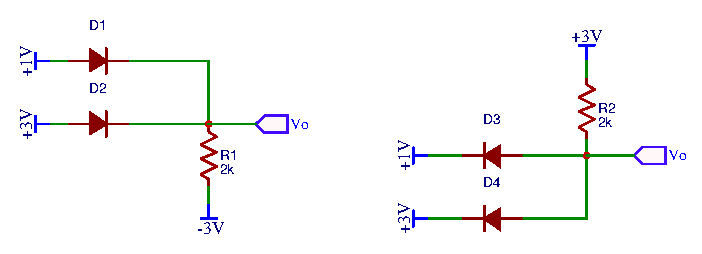
\includegraphics[scale=1.4]{ex3}
\end{center}
}
{%answer
Première partie de gauche à droite :
\begin{itemize}
    \item $V_o = -3V$ (diode passante) et $I = \frac{3-(-3)}{1k}=6mA$
    \item $V_o = 3V$ (diode bloquée) et $I=0A$
    \item $V_o = 3V$ (diode passante) et $I= \frac{3-(-3)}{1k}=6mA$
    \item $V_o = -3V$ (diode bloquée) et $I = 0A$
\end{itemize}
~\newline
Deuxième partie de gauche à droite :
\begin{itemize}
    \item $V_o = 3V$ (D1 bloquée et D2 passante) et $I = \frac{3-(-3)}{2k} = 3mA$
    \item $V_o = 1V$ (D3 passante et D4 bloquée) et $I = \frac{3-(+1)}{2k} = 1mA$
\end{itemize}

Reprenons le premier circuit de la seconde partie.
La circuit peut être redessiné de la façon suivante :
\begin{center}
    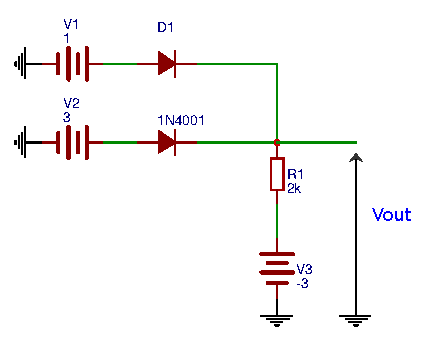
\includegraphics[scale=1.4]{ex3-corrige}
\end{center}

Pour résoudre un circuit à diodes, il faut poser l'hypothèse que chacune est soit bloquante, soit passante.
Les hypothèses menant à des incohérences sont ensuite éliminées.

\begin{enumerate}
    \item D1 et D2 sont passantes.

    Dans la maille comprenant les deux diodes, on a $1V - V_{D1} -V_{D2} - 3V = 0$.
    Les diodes étant passantes et idéales, leur tension est nulle, ce qui implique que $1V = 3V$, ce qui est incohérent.

    \item D1 et D2 sont bloquantes.

    Dans la maille comprenant D1 et R1, on a $1V - V_{D1} - i \cdot R1 - (-3V) = 0$.
    Les diodes étant bloquantes, il n'y a pas de courant qui circule dans le circuit, donc $V_{D1} = 4V$.
    Or, si D1 est bloquante et idéale, sa tension ne peut être positive.
    Les hypothèses sont à nouveau fausses.

    \item D1 est bloquante et D2 passante.

    Via la maille comprenant D2 et $V_o$, on trouve $V_o = 3V$.
    Pour déterminer le courant, on peut prendre la maille comprenant D2 et R1, ce qui donne $3V - i \cdot R1 - (-3V) = 0$, c'est-à-dire $i = \frac{6V}{2k\Omega} = 3mA$.
    Si l'on détermine tous les courants et toutes les tensions dans le circuit, on ne trouve aucune incohérence.
    Les hypothèses sont donc correctes, il n'est pas nécessaire de vérifier les autres combinaisons.
\end{enumerate}
}


\Question{
\label{sinus}
En considérant la diode comme idéale et $V_i$ comme une source de tension sinusoïdale de $1kHz$ et d'amplitude $5V$ centrée en $0V$, dessiner l'allure de la tension en sortie du montage $V_o$ pour les circuits suivants.
\begin{center}
    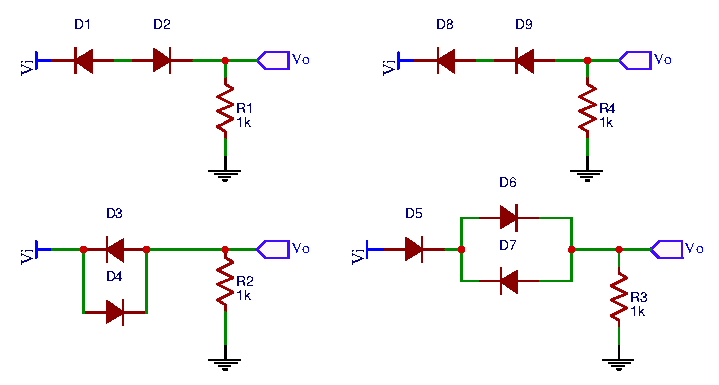
\includegraphics[scale=1.4]{ex4}
\end{center}

}
{%answer
De haut en bas et de gauche à droite :
    \begin{itemize}
        \item $V_o = 0V$ (rien en sortie)
        \item Uniquement les alternances négatives (jusqu'à -5V)
        \item Pas de changement sur le sinus (entre +5 et -5V)
        \item Uniquement les alternances positives (jusqu'à +5V)
    \end{itemize}
}

\Question{
Refaire les exercices \ref{conti} et \ref{sinus} en considérant la diode comme une mise en série d'une diode idéale et d'une source de tension de 0.7V.
}
{%answer
Pour le \ref{conti} :
Première partie de gauche à droite :
\begin{itemize}
    \item $V_0 = -2.3V$ (diode passante) et $I = \frac{3-(-2.3)}{1k}=5.3mA$
    \item $V_0 = 3V$ (diode bloquée) et $I=0A$
    \item $V_0 = 2.3V$ (diode passante) et $I= \frac{2.3-(-3)}{1k}=5.3mA$
    \item $V_0 = -3V$ (diode bloquée) et $I = 0A$
\end{itemize}
~\newline
Deuxième partie de gauche à droite :
\begin{itemize}
    \item $V_0 = 2.3V$ (D1 bloquée et D2 passante) et $I = \frac{2.3-(-3)}{2k} = 2.7mA$
    \item $V_0 = 1.7V$ (D3 passante et D4 bloquée) et $I = \frac{3-(+1.7)}{2k} = 0.65mA$
\end{itemize}

Pour le \ref{sinus} :
De haut en bas et de gauche à droite :
    \begin{itemize}
        \item $V_0 = 0V$ (rien en sortie)
        \item Uniquement les alternances négatives (jusqu'à -3.6V)
        \item Un sinus atténué (entre +4.3V et -4.3V)
        \item Uniquement les alternances positives mais atténuées (jusqu'à +3.6V)
    \end{itemize}

}

\Question{
Rappeler les schémas des redresseurs simple et double alternance.
}
{%answer
\begin{center}
    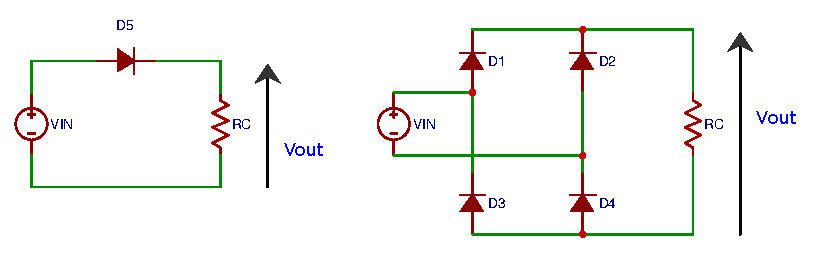
\includegraphics[width=\linewidth]{redr}
\end{center}
}

\Question{
Dessiner le schéma d'un montage permettant à l'aide d'une diode zener de produire une tension de $5.6V$ en sortie avec une entrée pouvant varier de $10V$ à $12V$ continu.
Dimensionner le circuit pour qu'il puisse délivrer au moins un courant de 100mA à la charge. Déterminer alors la puissance maximale dissipée par la diode.
}
{%answer
\begin{center}
    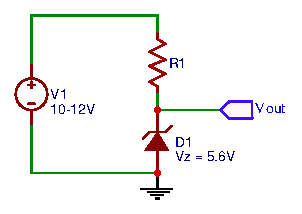
\includegraphics[width=6cm]{corexzener}
\end{center}
Un régulateur zener se compose de deux éléments~: une diode zener en parallèle de la charge permettant de limiter la tension, ainsi qu'une résistance permettant de limiter le courant.

Commençons par dimmensionner la résistance.
\begin{align*}
V_1 - R_1 \cdot i - 5.6V & = 0 \\
\Leftrightarrow i & = \frac{V_1 - 5.6V}{R_1} \geq 100 mA \\
\Leftrightarrow R_1 & \leq \frac{V_1 - 5.6V}{100 mA}
\end{align*}

Ainsi, pour $V_1 = 10 V$, on obtient $R_1 \leq 44 \Omega$.

% Augmenter $R1$ réduit la puissance dissipée par le régulateur ($=\left\lbrace R1, D1 \right\rbrace$). Néanmoins le maximum de R1 est déterminé par la tension d'entrée minimale et par le courant maximum en sortie (I).
% On veut $V_1 - I*R1 > 5.6$ donc si $V = 10V$ et $I=100mA$, on a $R1 < 44\Omega$.

La puissance dissipée par le régulateur est maximale quand la charge est infinie (tout le courant passe par la diode et le courant de sortie est nul) et la tension en entrée est de $12V$, on a alors : $I_{charge}=0$, $I_{R1,D1} = \frac{V_1 - Vz}{R1} = 145mA$ et donc $P_{Diode} = V_z \cdot I_D = 815mW$.
}

%\newpage
\Question{
Soit le circuit ci-dessous constitué d'une diode 1N4001, d'une LED NTE3019, de deux résistances de $10\Omega$ et d'une source de tension sinusoïdale
de $6V_{Cr\hat{e}te\:\grave{a}\:Cr\hat{e}te}$ à 50Hz.

\begin{center} 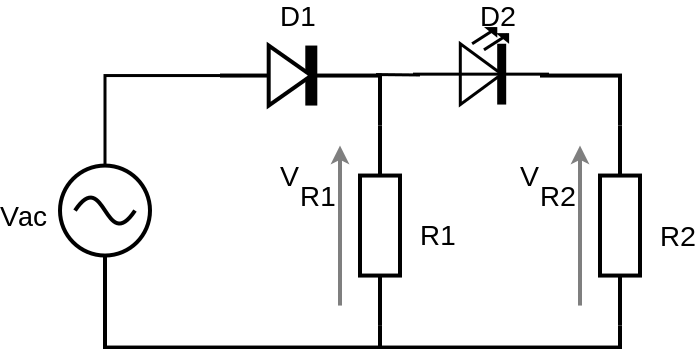
\includegraphics[width=300px]{diodes2.png} \end{center}

\ifgv{\newpage}
Sur base du schéma ci-dessus et en vous aidant des datasheets :
\begin{itemize}
    \item Tracer sur le graphique la tension aux bornes de $R1$ et celle aux bornes
de $R2$, pour $V_{ac}$ représentée.
    \item Indiquer les valeurs de tension remarquables et indiquez quand la LED s'allume.
    \item Quel est le courant maximum dans $R1$, dans la LED, dans $D1$ ?
    \item Quelle est la puissance dissipée par $D1$ ?
\end{itemize}

\ifthenelse{\boolean{corrige}}{}{\begin{center} 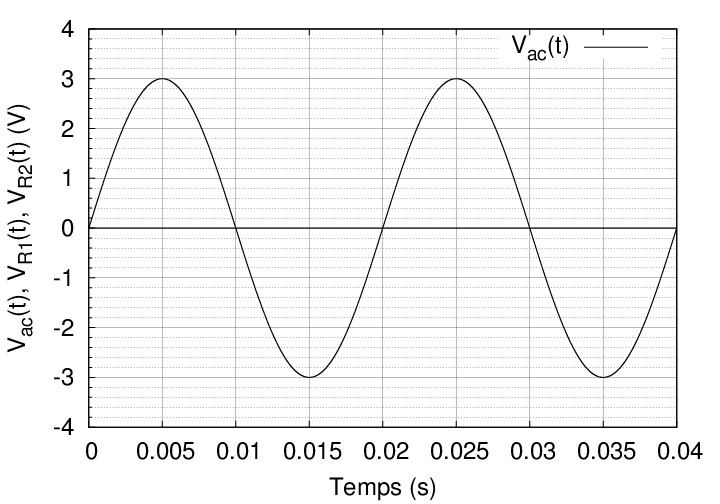
\includegraphics[width=300px]{image2.png} \end{center}}

}
{%answer
\begin{center} 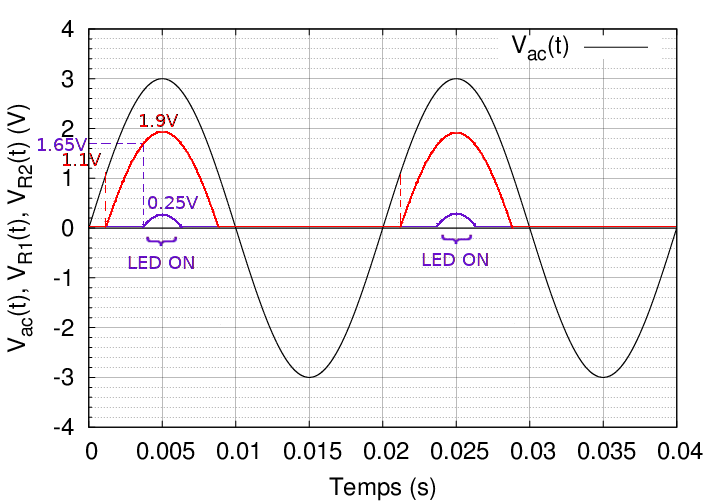
\includegraphics[width=300px]{image2corr.png} \end{center}
Les courants max sont :
\begin{itemize}
    \item $I_{R1} = \frac{1.9}{10} = 190mA$
    \item $I_{D2} = \frac{0.25}{10} = 25mA$
    \item $I_{D1} = I_{R1} + I_{D2} = 215mA$
\end{itemize}
La puissance dissipée par D1 est : $P_{D1} = U_{D1}*I_{D1} = 215mA*1.1V = 0.24W$
}
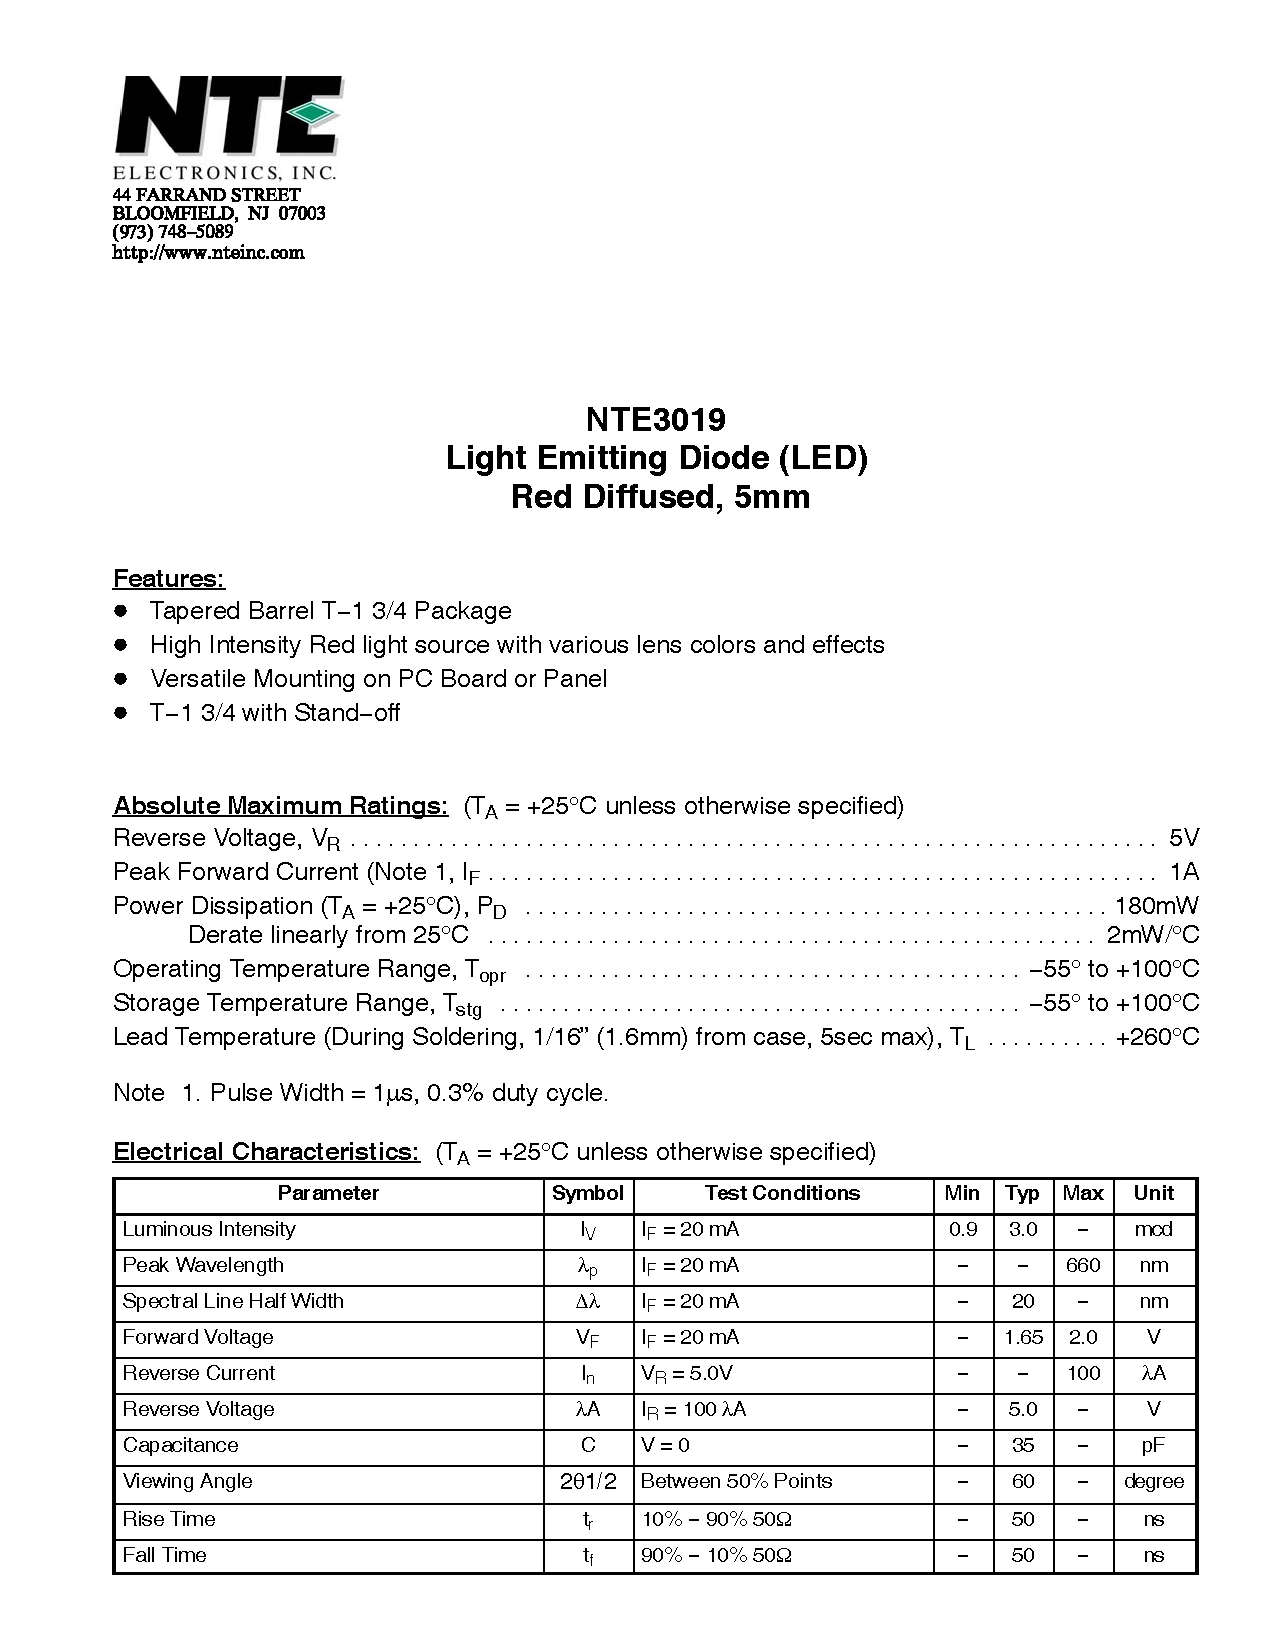
\includepdf[pages={1},scale=0.9,pagecommand={\pagestyle{plain}}]{nte3019.pdf}
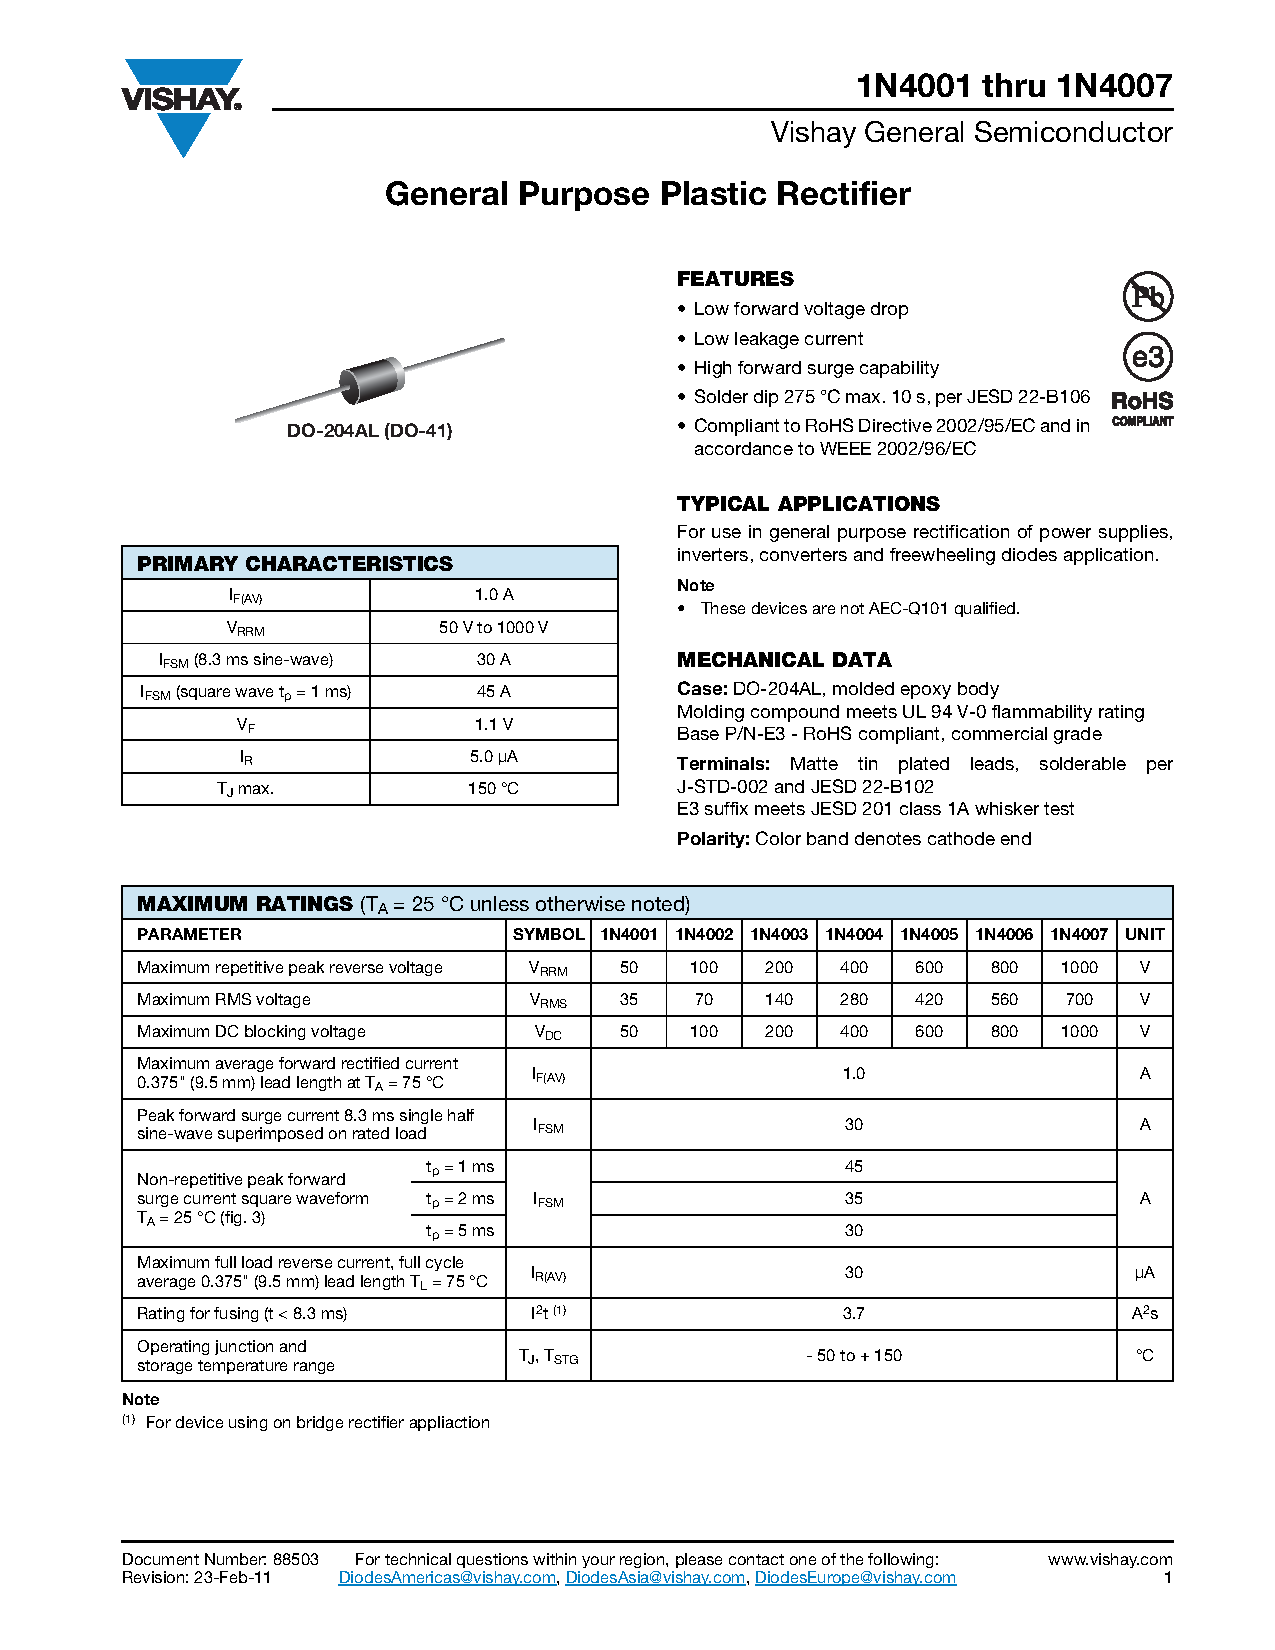
\includepdf[pages={1-2},scale=0.9,pagecommand={\pagestyle{plain}}]{1n4001.pdf}

\end{document}
